\documentclass[a4paper]{report}
\usepackage{listings}
\usepackage{enumitem}
\usepackage{mdframed}
\usepackage{graphicx} % Required for the inclusion of images
\usepackage{afterpage}

\title{CEEN 8886: Homework 6}
\date{2017-04-19}
\author{Kelly Boswell}

\makeatletter
\DeclareRobustCommand{\textsupsub}[2]{{%
  \m@th\ensuremath{%
    ^{\mbox{\fontsize\sf@size\z@#1}}%
    _{\mbox{\fontsize\sf@size\z@#2}}%
  }%
}}
\makeatother

\begin{document}

\maketitle

\pagenumbering{gobble}

\newpage

\pagenumbering{arabic}

% Problem 1
\section{Problem 1 --- 3G (UMTS) Security}

\subsection{Discuss the new infrastructure requirements in moving from a GSM
            network to UMTS.}

In GSM, the main architectural components are illustrated in Figure \ref{fig:prob1a}.
They are the Mobile Station (MS) which includes the subscriber's SIM card;
the Base Station Subsystem which consists of Base Station
Controller (BSC) and the Base Transceiver Station (BSS); and the Network Subsystem
which consists of the Home Location Register (HLR), the Visitor Location Register
(HLR), the Equipment Identity Register (EIR), the Authentication Centre (AuC), and
the Mobile Service Switching Center (MSC).

In UMTS, the main architectural components are illustrated in Figure \ref{fig:prob1b}
and Figure \ref{fig:prob1c}.  They are the User Equipment (UE) which includes the
users USIM card; the UMTS Terrestrial Radio Access Network (UTRAN) which is composed
of Node Bs used to connect the UE to a the core network via a Radio Network Controller
(RNC); and the core network which consists of the HLR, VLR, EIR, MSC, and AuC but includes
new components to support General Packet Radio Service (GPRS) --- intruduced in 2.5G --- 
for packet-based wireless communications to support TCP/IP communication protocols. These
new components are the Serving GPRS Support Node (SGSN) and the Gateway GPRS Support Node
(GGSN). The core network also consists of a Gateway Mobile Switching Centre (GMSC) used to
interface to external networks.

\afterpage{
\begin{figure}
\begin{mdframed}
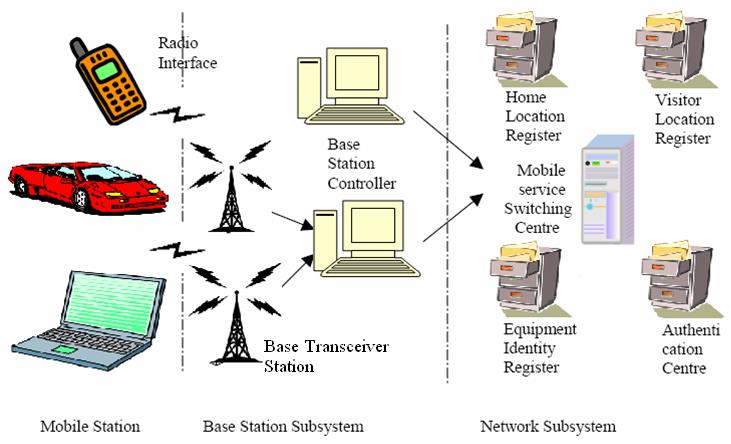
\includegraphics[scale=0.4]{GSM_Architecture.png}
\caption{GSM Architecture}
\label{fig:prob1a}
\end{mdframed}
\end{figure}
}

\afterpage{
\begin{figure}
\begin{mdframed}
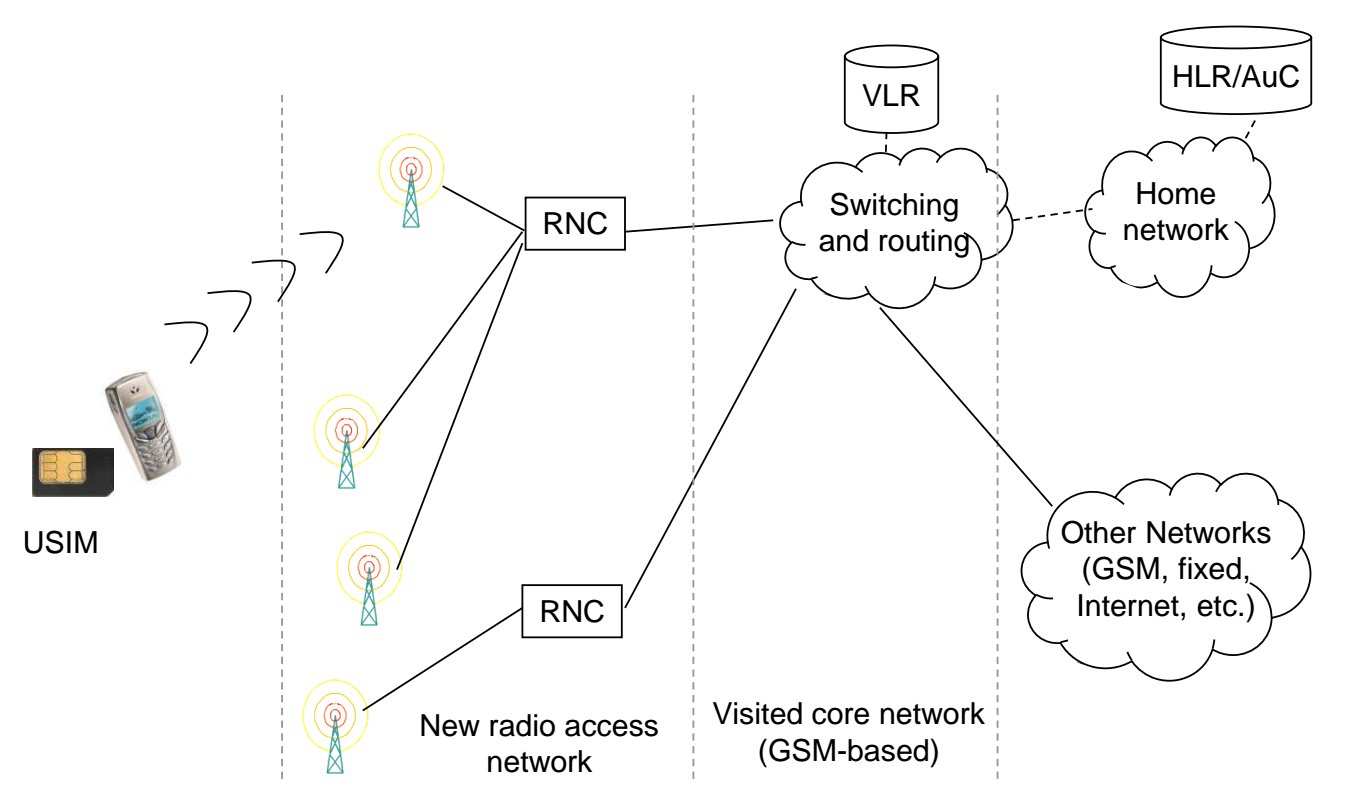
\includegraphics[scale=0.2]{UMTS_Architecture1.jpg}
\caption{3GPP Architecture --- UMTS}
\label{fig:prob1b}
\end{mdframed}
\end{figure}
}

\afterpage{
\begin{figure}
\begin{mdframed}
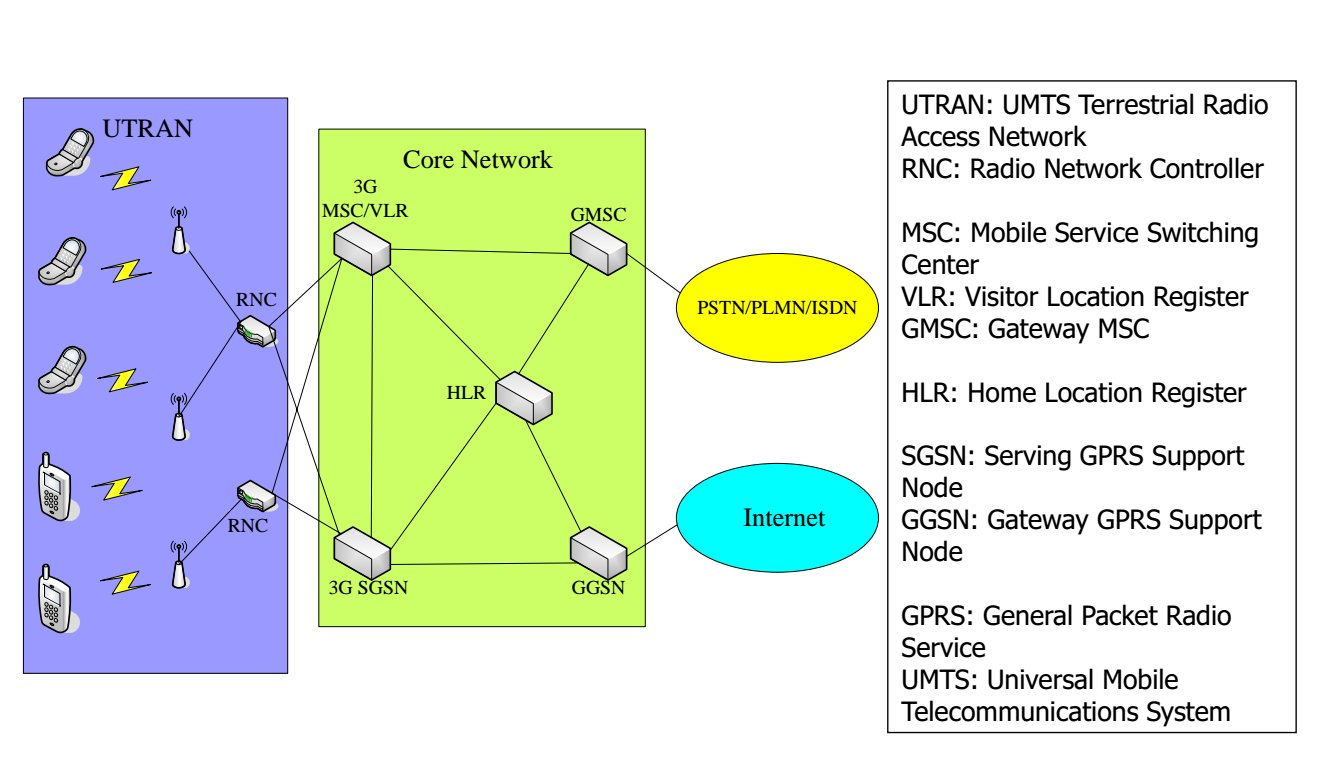
\includegraphics[scale=0.2]{UMTS_Architecture2.jpg}
\caption{3GPP Architecture --- UMTS}
\label{fig:prob1c}
\end{mdframed}
\end{figure}
}

%Problem 2
\section{Problem 2 --- LTE Security}

\subsection{Illustrate the improvements of LTE security over UMTS security.
            Give detailed explanations.}

\begin{enumerate}
\item Network Access Security
    \begin{enumerate}
    \item Refer to Figure \ref{fig:prob2a} for a depiction of UMTS Authentication and to Figure \ref{fig:prob2b} for a depiction
             of LTE Authentication and compare and contrast.
    \item Serving network identity (SN ID) has been added to the EPS AKA procedure to avoid attacks 
             such as redirection attacks and false base station attacks.
    \item On top of the security functions at the access stratum (AS) level between the User Equipment
             (UE) and the eNB, new security functions at the non access stratum (NAS) level between the 
             UE and the Mobility Management Entity (MME) have been included.
    \item The new root key K\textsubscript{ASME}, computed by the Home Server Subscriber (HSS), will be delivered
             to the Mobility Management Entity (MME) or the serving network (SN).
    \item The key set identifier KSI\textsubscript{ASME} is embedded in the user authentication request message
             transmitted to the UE by the MME.
    \item A new key heirarchy is introduced to protect the security of the signaling and user data traffic.
    \end{enumerate}
\item Security in Handover Processes
    \begin{enumerate}
    \item Intra E-UTRAN mobility: The current eNB and the target eNB are managed by the same MME
        \begin{enumerate}
        \item View Figure \ref{fig:prob2c} for a depiction of the Inter-eNB handover procedure.
        \item A new key management mechanism is designed with different ways to derive the new eNB keys
                 based on vertical or horizontal key derivations.
        \item A MME and the UE shall derive a K\textsubscript{eNB} and a next hop (NH) parameter from the K\textsubscript{ASME},
                 which is derived by the UE and the MME after an initial access authentication.
        \item In the initial setup, K\textsubscript{eNB} is derived directly from the K\textsubscript{ASME}, and is then associated with a
                 virtual NH parameter with a NH chaining counter (NCC)  value to be zero. The UE and the eNB
                 use the K\textsubscript{eNB} to secure the communication on the air interface.
        \item In handovers, a new session key used between the UE and the target eNB, K\textsupsub{*}{eNB},
                 is derived from either the active K\textsubscript{eNB} or from the NH parameter.
        \end{enumerate}
    \item Mobility between the E-UTRAN and UTRAN/GERAN
        \begin{enumerate}
        \item For the handover from the E-UTRAN to the UMTS Terrestrial Radio Access Network (UTRAN) or the
                 GSM EDGE Radio Access Network (GERAN):
            \begin{enumerate}
            \item the UE and the MME shall first derive a CK and IK from the K\textsubscript{ASME}
            \item upon receiving CK' || IK' with KSI' from the MME, the target Service GPRS Supporting Node (SGSN) and
                     the UE shall replace all stored parameters CK, IK, KSI, with CK', IK', and KSI'.
            \item the UE and the target SGSN shall use CK' and IK' to derive the General Packet Radio Service (GPRS)
                     K\textsubscript{c}.
            \end{enumerate}
        \item For the handover from the UTRAN/GERAN to the E-UTRAN:
            \begin{enumerate}
            \item The target MME shall derive K\textsupsub{'}{ASME} from CK and IK or GPRS K\textsubscript{c} received
                     from the SGSN.
            \item The UE shall also execute the above same procedure as the MME to derive K\textsupsub{'}{ASME}.
            \item The target MME and the UE shall derive K\textsubscript{eNB} and the corresponding NAS keys according
                     to the key heirarchy of LTE. 
            \end{enumerate}
        \end{enumerate}
    \item Mobility between E-UTRAN and non-3GPP access networks
        \begin{enumerate}
        \item There are several different mobility scenarios between heterogeneous access systems in the LTE networks:
            \begin{enumerate}
            \item Handovers from trusted or untrusted non-3GPP access networks to the E-UTRAN
            \item Handovers from the E-UTRAN to trusted or untrusted non-3GPP access networks
            \end{enumerate}
        \item The UE, the target access network and the EPC will implement a full access authentication procedure before
                 the UE handovers to the new access network.
        \item Different access authentication procedures will be executed in distinct mobility scenarios.
        \end{enumerate}
    \end{enumerate}
\item Security in IP Multimedia Subsystem (IMS)
    \begin{enumerate}
    \item Refer to Figure \ref{fig:prob2d} for an overview of security in IMS.
    \item A UE needs a new IMS Subscriber Identity Module (ISIM) located within the Universal Integrated Circuit Card (UICC)
             for multimedia services.
    \item The IMS authentication keys and functions at the user side shall be stored in the ISIM.
    \item The main architectural elements in the IMS are the Session Initiation Protocol (SIP) proxies, Call Service Control 
             Functions (CSCF), which consists of Proxies-CSCF (P-CSCF), Interrogating-CSCF (I-CSCF) and Serving-CSCF (S-CSCF).
    \item Receiving a request from an UE, the P-CSCF redirects and forwards the SIP messages to the I-CSCF within the UE?s
             home network. Then, I-CSCF contacts the HSS for an appropriate S-CSCF to forward the registration request to.
    \item Upon the receipt of the request, the S-CSCF contacts the HSS to obtain the user?s authentication data to authenticate the
             UE and provide the session control of the multimedia services.
    \item Once the UE has successfully established a security association with the network and a separate security association
             to the IMS, an access will be granted to multimedia service.
    \item The IMS security architecture includes a few different security associations and different requirements for the security protection
             for the IMS.
        \begin{enumerate}
        \item A mutual authentication. The S-CSCF represents the HSS to authenticate the UE.
        \item A security link and a security association between the UE and a P-CSCF.
        \item Security within the network domain by applying Network Domain Security (NDS)/IP.
        \end{enumerate}
    \item In order to access the multimedia services, LTE users have to be authenticated in both the LTE network layer and the IMS service
            layer.
        \begin{enumerate}
        \item An IM subscriber needs the mutual authentication with the LTE network by the EPS-AKA before the access to multimedia services.
        \item An IMS AKA is executed between the ISIM and the Home Network (HN) for authentication and key agreement for the IMS.
        \end{enumerate}
    \end{enumerate}
\item Security at HeNB --- a femtocell access point installed by a subscriber at a residence or small office to increase indoor coverage for
         voice and high speed data services --- includes five security features:
    \begin{enumerate}
    \item HeNB access security
    \item Network domain security
    \item HeNB service domain security
    \item UE access control domain security
    \item UE access security domain
    \end{enumerate}
\item Security in MTC --- Machine to Machine communication (M2C) --- which is a form of data communication between entities without 
         human interaction. MTC Security Architecture includes three security areas:
    \begin{enumerate}
    \item Security for the MTC between the MTC device and 3GPP network.
        \begin{enumerate}
        \item (A1) Security for the MTC between MTC device and the Radio Access Network, E-UTRAN/UTRAN/GERAN
        \item (A2) Security for the MTC between MTC device and the MME
        \item (A3) Security for the MTC between MTC device and the MTC-IWF for 3GPP access/ePDG for non-3GPP access
        \end{enumerate}
    \item Security for the MTC between the 3GPP network, the MTC server / MTC user, and the MTC application
        \begin{enumerate}
        \item (B1) Security for the MTC between the MTC server and the 3GPP network, which can be further divided into security aspects 
                 when the MTC server is within and outside the 3GPP network
        \item (B2) Security for the MTC between the MTC user, MTC application, and the 3GPP network
        \end{enumerate}
    \item Security for the MTC between the MTC server / MTC user, the MTC application, and the MTC device
        \begin{enumerate}
        \item (C1) Security for the MTC between the MTC server and the MTC device
        \item (C2) Security for the MTC between the MTC user, MTC application, and the MTC device
        \end{enumerate}
    \end{enumerate}
\end{enumerate}

\begin{figure}
\begin{mdframed}
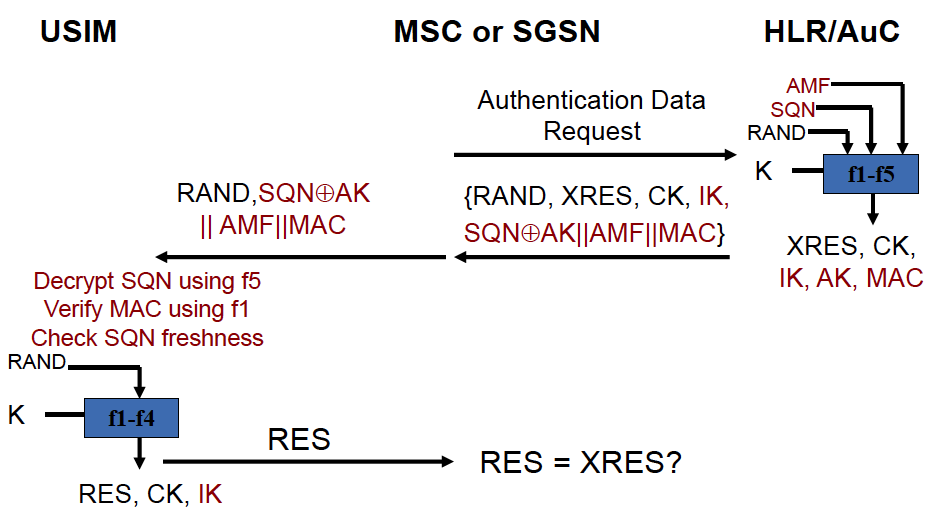
\includegraphics[scale=0.35]{UMTS_Authentication.png}
\caption{UMTS Authentication --- UMTS-AKA}
\label{fig:prob2a}
\end{mdframed}
\end{figure}

\begin{figure}
\begin{mdframed}
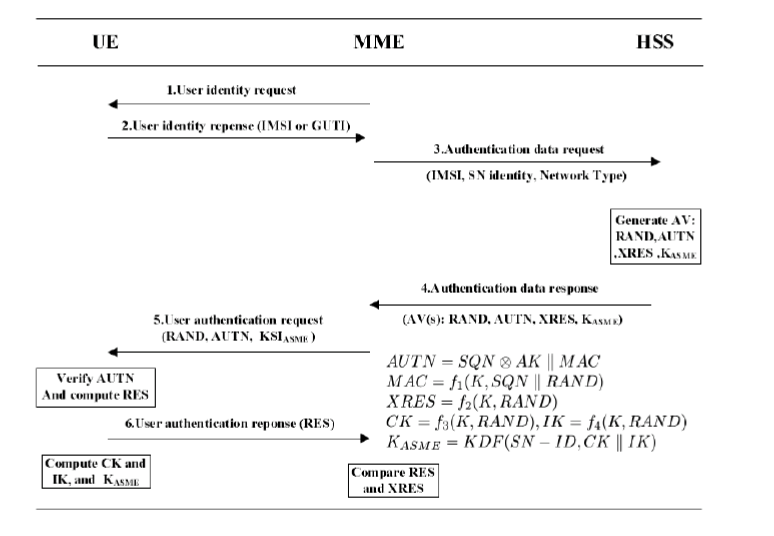
\includegraphics[scale=0.43]{LTE_Authentication.jpg}
\caption{LTE Authentication --- EPS-AKA}
\label{fig:prob2b}
\end{mdframed}
\end{figure}

\begin{figure}
\begin{mdframed}
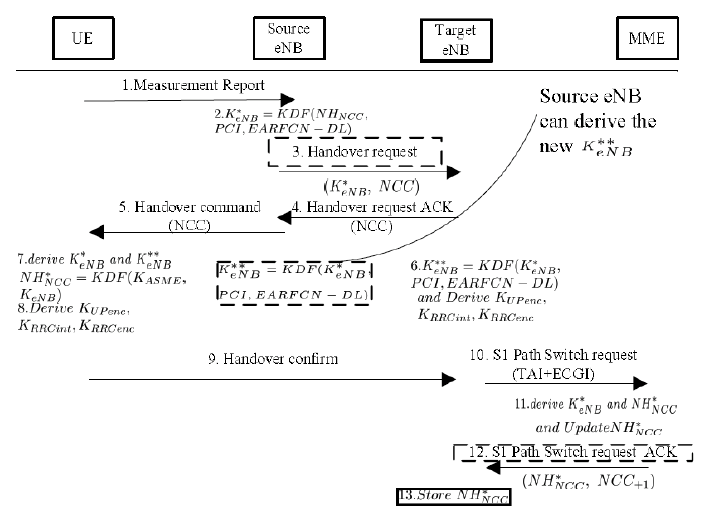
\includegraphics[scale=0.45]{Inter_eNB_Handover.png}
\caption{Inter-eNB Handover}
\label{fig:prob2c}
\end{mdframed}
\end{figure}

\begin{figure}
\begin{mdframed}
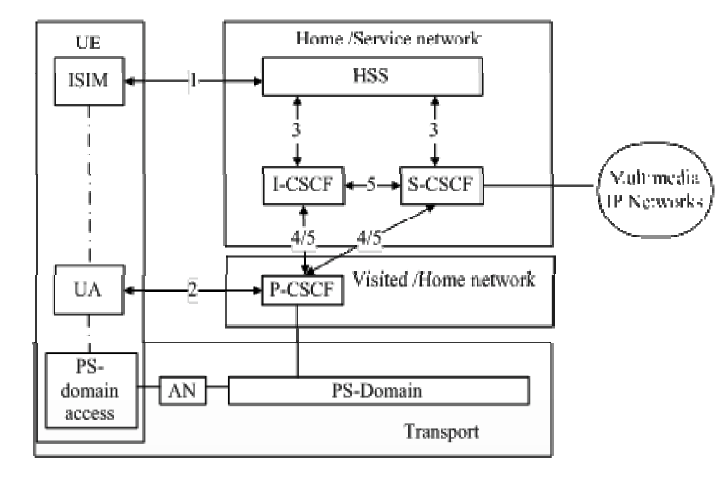
\includegraphics[scale=0.45]{IMS_Security.png}
\caption{Security in IMS}
\label{fig:prob2d}
\end{mdframed}
\end{figure}

%Problem 3
\section{Problem 3 --- IEEE 802.15 for WPAN Security}

\subsection{What is the hopping rate in Bluetooth and how many bits are
            transmitted in one slot transmission?}

The hopping rate in bluetooth is 1,600 hops per second. However, with adaptive frequency hopping
the rate may be reduced by 50\% or 800 hops per second.  The number of bits transmitted in a single
slot transmission may vary per packet type. Each time slot carries 240 bits of data. 

\subsection{Which 802.11 LAN standards will Bluetooth interfere with?}

Bluetooth devices may interfere with any 802.11 standard that is in the same frequency band of 2.4-GHz, namely 802.11 b/g/n.
Current versions use adaptive frequency hopping to mitigate interference, however.

\subsection{What is the reason for a lower speed/lower power WPAN standard
            such as IEEE 802.15.4?}

To support internetworking of low-power embedded devices, such as wireless sensor devices that are becoming ubiquitous
in the IoT consumer market.

\end{document}
